\section{QUY HOẠCH QUỸ ĐẠO TRAJECTORY PLANNING}
\subsection{Linear Segment with Parabolic Blend (\textit{LSPB})}
Xây dựng giải thuật LSPB
\begin{figure}[H]
	\centering
	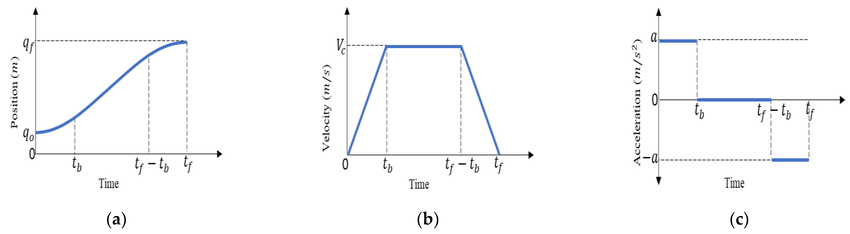
\includegraphics[width=1\linewidth]{Images/lspb.png}
	\caption{Linear Segment with Parabolic Blend}
	\label{fig:enter-label10}
\end{figure}

\vspace{0.5cm}
\begin{lstlisting}[language=python]
	def lspb(q0, qn, vmax, amax):
		if q0 == qn:
		return np.zeros(1), np.array([q0]), np.zeros(1), np.zeros(1)
		q0 = q0*180/pi
		qn = qn*180/pi
		qmax = qn-q0
		if qmax < 0:
		amax = -amax
		vmax = -vmax
		t1 = round((vmax/amax)/0.0333)*0.0333
		
		if abs(qmax) < abs(amax*t1**2):
		t1 = round(np.sqrt(0.333*qmax*2/amax)/0.0333)*0.0333
		t2 = round(((qmax-amax*t1**2)/(amax*t1))/0.0333)*0.0333 + t1
		t3 = t2+t1
		
		else:
		t2 = round(((qmax-amax*t1**2)/vmax)/0.0333)*0.0333 + t1
		t3 = t2+t1
		
		t = np.arange(0, t3, 0.0333)
		
		qt = np.zeros(len(t), dtype=float)
		vt = np.zeros(len(t), dtype=float)
		at = np.zeros(len(t), dtype=float)
		
		for i, tt in enumerate(t):
		if tt <= t1:
		at[i] = amax
		vt[i] = at[i]*tt
		qt[i] = q0 + 0.5*at[i]*tt**2
		elif tt <= t2:
		at[i] = 0
		vt[i] = amax*t1
		qt[i] = q0 + 0.5*amax*t1**2 + vt[i]*(tt-t1)
		else:
		at[i] = -amax
		vt[i] = amax*t1 + at[i]*(tt-t2)
		qt[i] = q0 + 0.5*amax*t1**2 + amax*t1*(t2-t1) + amax*t1*(tt-t2) - 0.5*amax*(tt-t2)**2
		qt[-1] = qn
		vt[-1] = 0
		return t, qt*pi/180, vt, at
\end{lstlisting}


\subsection{Kết quả chạy được}
\begin{figure}[H]
	\centering
	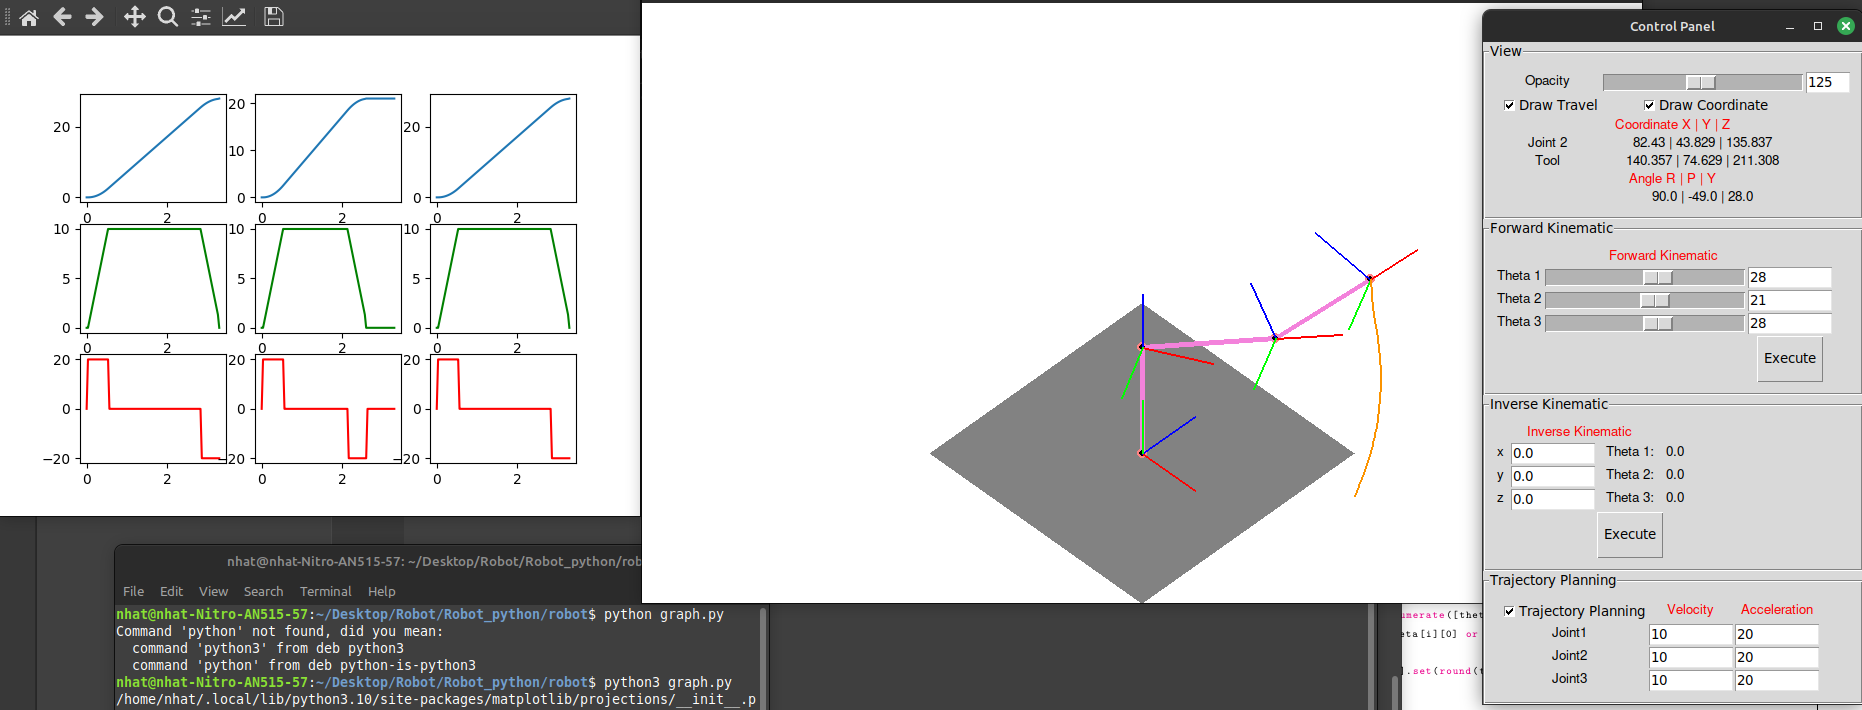
\includegraphics[width=1\linewidth]{Images/demo_trajectory.png}
	\caption{Linear Segment with Parabolic Blend}
	\label{fig:enter-label11}
\end{figure}